% Source for the figure of the multiplicative hashing (sec. 7.3.3): the
% product z x modulo 2^w and its top d bits, w = 16 and d = 4.
% Build: make figures (in ../build).
\documentclass[border=4pt]{standalone}
\usepackage[T1]{fontenc}
\usepackage{lmodern}
\usepackage{amsmath,amssymb}
\usepackage{tikz}
\usepackage{lamalunga}
% tikz-ads.tex: the TikZ styles shared by the figures of the memory of the
% manual, \input by each standalone figure: a cell of a vector (cell), the
% cell that an operation touches (touched), a free cell (free), a node of a
% linked structure (node), the labels of indices (index) and of variables
% (var), a pointer (ptr), and \cells and \indices to draw a row of cells.
\usetikzlibrary{arrows.meta,positioning,calc,fit,shapes.multipart}
\definecolor{adsTouched}{RGB}{214,196,236}
\definecolor{adsFree}{RGB}{236,236,236}
\tikzset{
  ads/.style={>={Stealth[length=2mm]},font=\small,
              every node/.append style={inner sep=0pt}},
  cell/.style={draw,minimum width=7mm,minimum height=7mm,
               font=\small\ttfamily,outer sep=0pt},
  touched/.style={cell,fill=adsTouched},
  free/.style={cell,fill=adsFree,text=black!45},
  node/.style={draw,rounded corners=1pt,minimum width=8mm,
               minimum height=6mm,font=\small\ttfamily},
  index/.style={font=\scriptsize\ttfamily,text=black!60},
  var/.style={font=\small\itshape},
  ptr/.style={->,thick}
}
% \cells{name}{x,y}{list}: a row of cells, the first at (x,y), named
% name-0, name-1, ...; each item is text/style, the style one of cell,
% touched and free (e.g., {a/cell,e/touched,/free})
\newcommand{\cells}[3]{%
  \foreach \v/\s [count=\i from 0] in {#3}
    \node[\s] (#1-\i) at ($(#2)+(\i*7mm,0)$) {\v};}
% \indices{name}{n}: the indices 0 .. n-1 under the cells of name
\newcommand{\indices}[2]{%
  \foreach \i in {0,...,\numexpr#2-1\relax}
    \node[index,below=1.2mm of #1-\i] {\i};}

\tikzset{bit/.style={cell,minimum width=4.4mm,minimum height=5.4mm,
           font=\scriptsize\ttfamily,line width=0.8pt},
         bitfree/.style={free,minimum width=4.4mm,minimum height=5.4mm,
           font=\scriptsize\ttfamily,line width=0.8pt},
         bittouched/.style={touched,minimum width=4.4mm,minimum height=5.4mm,
           font=\scriptsize\ttfamily\bfseries,line width=0.8pt}}
\newcommand{\brow}[3]{% name, y, list; right aligned at column 21
  \def\nb{0}\foreach \v/\s in {#3} {\xdef\nb{\the\numexpr\nb+1\relax}}%
  \foreach \v/\s [count=\i from 0] in {#3}
    \node[\s] (#1-\i) at ($(0,#2)+({(\i+22-\nb)*4.6mm},0)$) {\v};}
\newcommand{\ry}[1]{\ifcase#1\or0mm\or-7mm\or-14mm\or-21mm\or-28mm\or-35mm\fi}
\begin{document}
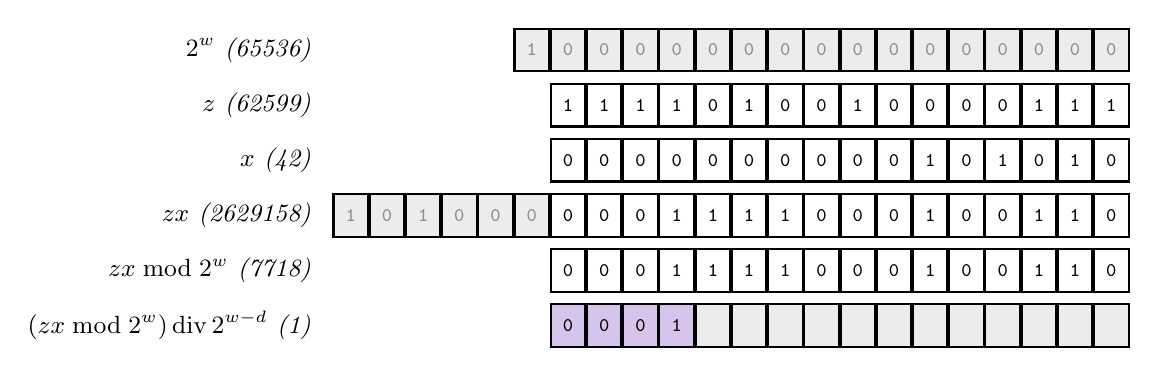
\begin{tikzpicture}[ads]
  \tikzset{lab/.style={var,anchor=east}}
  \brow{r1}{0}{1/bitfree,0/bitfree,0/bitfree,0/bitfree,0/bitfree,0/bitfree,0/bitfree,0/bitfree,0/bitfree,0/bitfree,0/bitfree,0/bitfree,0/bitfree,0/bitfree,0/bitfree,0/bitfree,0/bitfree}
  \node[lab] at (-5mm,\ry{1}) {$2^w$ (65536)};
  \brow{r2}{-7mm}{1/bit,1/bit,1/bit,1/bit,0/bit,1/bit,0/bit,0/bit,1/bit,0/bit,0/bit,0/bit,0/bit,1/bit,1/bit,1/bit}
  \node[lab] at (-5mm,\ry{2}) {$z$ (62599)};
  \brow{r3}{-14mm}{0/bit,0/bit,0/bit,0/bit,0/bit,0/bit,0/bit,0/bit,0/bit,0/bit,1/bit,0/bit,1/bit,0/bit,1/bit,0/bit}
  \node[lab] at (-5mm,\ry{3}) {$x$ (42)};
  \brow{r4}{-21mm}{1/bitfree,0/bitfree,1/bitfree,0/bitfree,0/bitfree,0/bitfree,0/bit,0/bit,0/bit,1/bit,1/bit,1/bit,1/bit,0/bit,0/bit,0/bit,1/bit,0/bit,0/bit,1/bit,1/bit,0/bit}
  \node[lab] at (-5mm,\ry{4}) {$z x$ (2629158)};
  \brow{r5}{-28mm}{0/bit,0/bit,0/bit,1/bit,1/bit,1/bit,1/bit,0/bit,0/bit,0/bit,1/bit,0/bit,0/bit,1/bit,1/bit,0/bit}
  \node[lab] at (-5mm,\ry{5}) {$z x \bmod 2^w$ (7718)};
  \brow{r6}{-35mm}{0/bittouched,0/bittouched,0/bittouched,1/bittouched,/bitfree,/bitfree,/bitfree,/bitfree,/bitfree,/bitfree,/bitfree,/bitfree,/bitfree,/bitfree,/bitfree,/bitfree}
  \node[lab] at (-5mm,\ry{6})
    {$( z x \bmod 2^w ) \operatorname{div} 2^{w-d}$ (1)};
\end{tikzpicture}
\end{document}
